\let\negmedspace\undefined
\let\negthickspace\undefined
\documentclass[journal]{IEEEtran}
\usepackage[a5paper, margin=10mm, onecolumn]{geometry}
%\usepackage{lmodern} % Ensure lmodern is loaded for pdflatex
\usepackage{tfrupee} % Include tfrupee package

\setlength{\headheight}{1cm} % Set the height of the header box
\setlength{\headsep}{0mm}     % Set the distance between the header box and the top of the text

\usepackage{gvv-book}
\usepackage{gvv}
\usepackage{cite}
\usepackage{amsmath,amssymb,amsfonts,amsthm}
\usepackage{algorithmic}
\usepackage{graphicx}
\usepackage{textcomp}
\usepackage{xcolor}
\usepackage{txfonts}
\usepackage{listings}
\usepackage{enumitem}
\usepackage{mathtools}
\usepackage{gensymb}
\usepackage{comment}
\usepackage[breaklinks=true]{hyperref}
\usepackage{tkz-euclide} 
\usepackage{listings}
% \usepackage{gvv}                                        
\def\inputGnumericTable{}                                 
\usepackage[latin1]{inputenc}                                
\usepackage{color}                                            
\usepackage{array}                                            
\usepackage{longtable}                                       
\usepackage{calc}                                             
\usepackage{multirow}                                         
\usepackage{hhline}                                           
\usepackage{ifthen}                                           
\usepackage{lscape}
\begin{document}

\bibliographystyle{IEEEtran}
\vspace{3cm}

\title{2019-PH-27-39}
\author{EE24BTECH11066 - YERRA AKHILESH
}
% \maketitle
% \newpage
% \bigskip
{\let\newpage\relax\maketitle}

\renewcommand{\thefigure}{\theenumi}
\renewcommand{\thetable}{\theenumi}
\setlength{\intextsep}{10pt} % Space between text and floats


\numberwithin{equation}{enumi}
\numberwithin{figure}{enumi}
\renewcommand{\thetable}{\theenumi}
\begin{enumerate}[start=27]
\item Consider a three-dimensional crystal of $N$ inert gas atoms. The total energy is given by $U\brak{R}=2N \in \sbrak{p\brak{\frac{\sigma}{R}}^{12}-q\brak{\frac{\sigma}{R}}^{6}}$, where $p=12.13, q=14.45$, and $R$ is the nearest neighbour distance between two atoms. The two constants, $\in$ and $R$, have the dimensions of energy and length, respectively. The equilibrium separation between two nearest neighbour atoms in units of $\sigma \brak{\text{rounded off to two decimal places}}$ is \underline{\hspace{1cm}} \hfill{[2019-PH]}\\
%28
\item The energy-wavevector $\brak{E-k}$ dispersion relation for a particle in two dimensions is $E=Ck$, where $C$ is a constant. If its density of states $D\brak{E}$ is proportional to $E^p$ then the value of $p$ is \underline{\hspace{1cm}} \hfill{[2019-PH]}\\
%29
\item A circular loop made of a thin wire has radius $2$ cm and resistance $2\ohm$. It is placed perpendicular to a uniform magnetic field of magnitude $\abs{\overrightarrow{B}_0}=0.01$ Tesla. At time $t=0$ the field starts decaying as $\overrightarrow{B}=\overrightarrow{B}_0 e^{\frac{-t}{t_{0}}}$, where $t_{0}=1s$. The total charge that passes through a cross section of the wire during the decay is $Q$. The value of $Q$ in $\mu C \brak{\text{rounded off to two decimal places}}$ is \underline{\hspace{1cm}} \hfill{[2019-PH]}\\
%30
\item The electric field of an electromagnetic wave in vacuum is given by \\
\begin{align*}
    \overrightarrow{E}=E_{0} \cos \brak{3y+4z-1.5 \times 10^{9} t} \hat{x}.
\end{align*}
The wave is reflected from the $z=0$ surface. If the pressure exerted on the surface is $\alpha\in_{0}E_0^{2}$, the value of $\alpha \brak{\text{rounded off to one decimal place}}$ is  \underline{\hspace{1cm}} \hfill{[2019-PH]}\\
%31
\item The Hamiltonian for a quantum harmonic oscillator of mass $m$ in three dimensions is \\
\begin{align*}
    H=\frac{p^{2}}{2m}+\frac{1}{2}m \omega^{2}r^{2}
\end{align*}
where $\omega$ is the angular frequency. The expectation value of $r^{2}$ in the first excited state of the oscillator in units of $\frac{\hbar}{m\omega} \brak{\text{rounded off to one decimal place}}$
is \underline{\hspace{1cm}}

    \hfill{[2019-PH]}\\
%32
\item The Hamiltonian for a particle of mass $m$ is $H=\frac{p^{2}}{2m}+kqt$ where $q$ and $p$ are the generalized coordinate and momentum, respectively, $t$ is time and $k$ is a constant. For the initial condition, $q=0$ and $p=0$ at $t=0, q\brak{t} \propto t^\alpha$. The value of $\alpha$ is \underline{\hspace{1cm}} \hfill{[2019-PH]}\\
%33
\item At temperature $T$Kelvin $\brak{K}$, the value of the Fermi function at an energy $0.5eV$ above the Fermi energy is $0.01$. Then $T$, to the nearest integer, is \underline{\hspace{1cm}}
$\brak{k_B=8.62 \times 10^{-5} \frac{eV}{K}}$ \hfill{[2019-PH]}\\
%34
\item Let $|\psi_1\rangle=\myvec{1\\0}, |\psi_2 \rangle=\myvec{0\\1}$ represent two possible states of a two-level quantum system. The state obtained by the incoherent superposition of $|\psi_1\rangle$ and $|\psi_2\rangle$ is given by a density matrix that is defined as $\rho \equiv c_1|\psi_1\rangle \langle\psi_1|+c_2|\psi_2\rangle \langle\psi_2|$. If $c_1=0.4$ and $c_2=0.6$, the matrix element $\rho_{22} \brak{\text{rounded off to one decimal place}}$ is \underline{\hspace{1cm}} 

    \hfill{[2019-PH]}\\
%35
\item A conventional type-I superconductor has a critical temperature of $4.7$K at zero magnetic field and a critical magnetic field of $0.3$ Tesla at $0$ K. The critical field in Tesla at $2$ K
$\brak{\text{rounded off to three decimal places}}$ is \underline{\hspace{1cm}} \hfill{[2019-PH]}\\
%36
\item Consider the following Boolean expression:\\
\begin{align*}
    \brak{\overline{A}+\overline{B}} \sbrak{\overline{A \brak{B+C}}} + A\brak{\overline{B}+\overline{C}}
\end{align*}
It can be represented by a single three-input logic gate. Identify the gate. \hfill{[2019-PH]}\\
\begin{enumerate}
\begin{multicols}{4}
\item AND
\item OR
\item XOR
\item NAND
\end{multicols}
\end{enumerate}
%37
\item The value of the integral $\int \limits_{-\infty}^{\infty} \frac{\cos \brak{kx}}{x^2+a^2}\, \text{dx}$, where $k>0$ and $a>0$, is \hfill{[2019-PH]}\\
\begin{enumerate}
\begin{multicols}{4}
\item $\frac{\pi}{a} e^{-ka}$
\item $\frac{2\pi}{a} e^{-ka}$
\item $\frac{\pi}{2a} e^{-ka}$
\item $\frac{3\pi}{2a} e^{-ka}$
\end{multicols}
\end{enumerate}
%38
\item The wave function $\psi\brak{x}$ of a particle is as shown below\\
\begin{figure}[H]
    \centering
    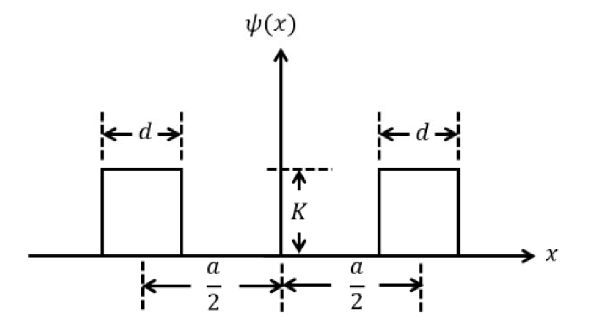
\includegraphics[width=0.5\linewidth]{figs/Figure_1.png}
    \label{fig:enter-label}
\end{figure}
Here $K$ is a constant, and $a>d$. The position uncertainty $\langle \Delta x \rangle$ of the particle is 

    \hfill{[2019-PH]}\\
\begin{enumerate}
\begin{multicols}{4}
\item $\sqrt{\frac{a^2 + 3d^2}{12}}$
\item $\sqrt{\frac{3a^2 + d^2}{12}}$
\item $\sqrt{\frac{d^2}{6}}$
\item $\sqrt{\frac{d^2}{24}}$
\end{multicols}
\end{enumerate}
%39
\item A solid cylinder of radius $R$ has total charge $Q$ distributed uniformly over its volume. It is rotating about its axis with angular speed $\omega$. The magnitude of the total magnetic moment of the cylinder is \hfill{[2019-PH]}\\
\begin{enumerate}
\begin{multicols}{2}
\item $QR^2 \omega$
\item $\frac{1}{2}QR^2 \omega$
\item $\frac{1}{4}QR^2 \omega$
\item $\frac{1}{8}QR^2 \omega$
\end{multicols}
\end{enumerate}

\end{enumerate}
\end{document}
